%!TEX program = lualatex
%
% Main document
% ===========================================================================
% This is part of the document "Project documentation template".
% Authors: brd3, kaa1
%

%---------------------------------------------------------------------------
\documentclass[
	a4paper,					% paper format
	10pt,							% fontsize
	twoside,					% double-sided
	openright,				% begin new chapter on right side
	notitlepage,			% use no standard title page
	parskip=half,			% set paragraph skip to half of a line
]{scrreprt}					% KOMA-script report
%---------------------------------------------------------------------------

\raggedbottom
\KOMAoptions{cleardoublepage=plain}			% Add header and footer on blank pages


% Load Standard Packages:
%---------------------------------------------------------------------------
\usepackage[standard-baselineskips]{cmbright}

\usepackage[english]{babel}										% english hyphenation
%\usepackage[latin1]{inputenc}  							% Unix/Linux - load extended character set (ISO 8859-1)
%\usepackage[ansinew]{inputenc}  							% Windows - load extended character set (ISO 8859-1)
\usepackage[T1]{fontenc}											% hyphenation of words with �,� and �
\usepackage{textcomp}													% additional symbols
\usepackage{ae}																% better resolution of Type1-Fonts
\usepackage{fancyhdr}													% simple manipulation of header and footer
\usepackage{etoolbox}													% color manipulation of header and footer
\usepackage{graphicx}                      		% integration of images
\usepackage{float}														% floating objects
\usepackage{caption}													% for captions of figures and tables
\usepackage{booktabs}													% package for nicer tables
\usepackage{tocvsec2}													% provides means of controlling the sectional numbering
%---------------------------------------------------------------------------

% Load Math Packages
%---------------------------------------------------------------------------
\usepackage{amsmath}                    	   	% various features to facilitate writing math formulas
\usepackage{amsthm}                       	 	% enhanced version of latex's newtheorem
\usepackage{amsfonts}                      		% set of miscellaneous TeX fonts that augment the standard CM
\usepackage{amssymb}													% mathematical special characters
\usepackage{exscale}													% mathematical size corresponds to textsize
%---------------------------------------------------------------------------

% Package to facilitate placement of boxes at absolute positions
%---------------------------------------------------------------------------
\usepackage[absolute]{textpos}
\setlength{\TPHorizModule}{1mm}
\setlength{\TPVertModule}{1mm}
%---------------------------------------------------------------------------

% Definition of Colors
%---------------------------------------------------------------------------
\RequirePackage{color}                          % Color (not xcolor!)
\definecolor{linkblue}{rgb}{0,0,0.8}            % Standard
\definecolor{darkblue}{rgb}{0,0.08,0.45}        % Dark blue
\definecolor{bfhgrey}{rgb}{0.41,0.49,0.57}      % BFH grey
%\definecolor{linkcolor}{rgb}{0,0,0.8}     			% Blue for the web- and cd-version!
\definecolor{linkcolor}{rgb}{0,0,0}        			% Black for the print-version!
%---------------------------------------------------------------------------

% Hyperref Package (Create links in a pdf)
%---------------------------------------------------------------------------
\usepackage[
	pdftex,ngerman,bookmarks,plainpages=false,pdfpagelabels,
	backref = {false},										% No index backreference
	colorlinks = {true},                  % Color links in a PDF
	hypertexnames = {true},               % no failures "same page(i)"
	bookmarksopen = {true},               % opens the bar on the left side
	bookmarksopenlevel = {0},             % depth of opened bookmarks
	pdftitle = {Template für Bachelor Thesis},	   	% PDF-property
	pdfauthor = {brd3},        					  % PDF-property
	pdfsubject = {LaTeX Template},        % PDF-property
	linkcolor = {linkcolor},              % Color of Links
	citecolor = {linkcolor},              % Color of Cite-Links
	urlcolor = {linkcolor},               % Color of URLs
]{hyperref}
%---------------------------------------------------------------------------

% Set up page dimension
%---------------------------------------------------------------------------
\usepackage{geometry}
\geometry{
	a4paper,
	left=28mm,
	right=15mm,
	top=30mm,
	headheight=20mm,
	headsep=10mm,
	textheight=242mm,
	footskip=15mm
}
%---------------------------------------------------------------------------

% Makeindex Package
%---------------------------------------------------------------------------
\usepackage{makeidx}                         		% To produce index
\makeindex                                    	% Index-Initialisation
%---------------------------------------------------------------------------

% Glossary Package
%---------------------------------------------------------------------------
% the glossaries package uses makeindex
% if you use TeXnicCenter do the following steps:
%  - Goto "Ausgabeprofile definieren" (ctrl + F7)
%  - Select the profile "LaTeX => PDF"
%  - Add in register "Nachbearbeitung" a new "Postprozessoren" point named Glossar
%  - Select makeindex.exe in the field "Anwendung" ( ..\MiKTeX x.x\miktex\bin\makeindex.exe )
%  - Add this [ -s "%tm.ist" -t "%tm.glg" -o "%tm.gls" "%tm.glo" ] in the field "Argumente"
%
% for futher informations go to http://ewus.de/tipp-1029.html
%---------------------------------------------------------------------------
\usepackage[nonumberlist]{glossaries}
\makeglossaries

\newglossaryentry{BibTeX}{name={BibTeX},description={Program for the creation of 	bibliographical references and directories in \TeX or \LaTeX documents}}
\newglossaryentry{Index}{name={Index},description={Index with keywords from text}}

\newglossaryentry{tls}{name={TLS},description={Trasport Layer Security}}
\newglossaryentry{dtls}{name={DTLS},description={Datagram Trasport Layer Security}}
\newglossaryentry{ae}{name={AE},description={Authenticated Encryption}}
\newglossaryentry{rfc}{name={RFC},description={Request for Comments}}
\newglossaryentry{ake}{name={AKE},description={Authenticated Key Etablishment}}
\newglossaryentry{ssl}{name={SSL},description={Secure Socket Layer}}
\newglossaryentry{tcp}{name={TCP},description={Transmission Control Protocol}}
\newglossaryentry{ip}{name={IP},description={Internet Protocol}}
\newglossaryentry{osi}{name={OSI},description={Open Systems Interconnection}}
\newglossaryentry{http}{name={HTTP},description={Hypertext Transfer Protocol}}
\newglossaryentry{https}{name={HTTPS},description={Hypertext Transfer Protocol Secure}}
\newglossaryentry{ftp}{name={FTP},description={File Transfer Protocol}}
\newglossaryentry{ftps}{name={FTPS},description={File Transfer Protocol Secure}}
\newglossaryentry{smtp}{name={SMTP},description={Simple Mail Transfer Protocol}}
\newglossaryentry{smtps}{name={SMTPS},description={Simple Mail Transfer Protocol Secure}}
\newglossaryentry{pop}{name={POP3},description={Post Office Protocol version 3}}
\newglossaryentry{pops}{name={POP3S},description={Post Office Protocol version 3 Secure}}
\newglossaryentry{pki}{name={PKI},description={Public Key Infrastructure}}
\newglossaryentry{mac}{name={MAC},description={Message Authentication Code}}
\newglossaryentry{ecdh}{name={(EC)DH},description={(Elliptic curve) Diffie-Hellman}}
\newglossaryentry{psk}{name={PSK},description={Pre-Shared Key}}
\newglossaryentry{dh}{name={DH},description={Diffie-Hellman}}
\newglossaryentry{dss}{name={DSS},description={Digital Signature Standard}}
\newglossaryentry{rsa}{name={RSA},description={Rivest–Shamir–Adleman cryptosystem}}
\newglossaryentry{ecdhe}{name={ECDHE},description={Elliptic curve Diffie-Hellman Ephemeral}}
\newglossaryentry{dhe}{name={DHE},description={Diffie-Hellman Ephemeral}}
\newglossaryentry{eddsa}{name={EdDSA},description={Edwards-curve Digital Signature Algorithm}}
\newglossaryentry{ecdsa}{name={ECDSA},description={Elliptic Curve Digital Signature Algorithm}}
\newglossaryentry{aead}{name={AEAD},description={Authenticated Encryption with Associated Data}}
\newglossaryentry{rcv}{name={RC4},description={Rivest Cipher 4}}


\newglossaryentry{rtt}{name={RTT},description={Round Trip Time}}


%---------------------------------------------------------------------------

% Intro:
%---------------------------------------------------------------------------
\begin{document}                              	% Start Document
\settocdepth{section}														% Set depth of toc
\pagenumbering{roman}
%---------------------------------------------------------------------------

\providecommand{\heading}{Internet Security - Transport Layer\\Comparative Study: TLS 1.2 VS TLS 1.3 }
					% Titel der Arbeit aus Datei titel.tex lesen
\providecommand{\versionnumber}{1.2}			%  Hier die aktuelle Versionsnummer eingeben
\providecommand{\versiondate}{02.01.2019}		%  Hier das Datum der aktuellen Version eingeben				% Versionsnummer und -datum aus Datei version.tex lesen

% Set up header and footer
%---------------------------------------------------------------------------
\makeatletter
\patchcmd{\@fancyhead}{\rlap}{\color{bfhgrey}\rlap}{}{}		% new color of header
\patchcmd{\@fancyfoot}{\rlap}{\color{bfhgrey}\rlap}{}{}		% new color of footer
\makeatother

\fancyhf{}																		% clean all fields
\fancypagestyle{plain}{												% new definition of plain style
	\fancyfoot[OR,EL]{\footnotesize \thepage} 	% footer right part --> page number
	\fancyfoot[OL,ER]{\footnotesize \heading, Version \versionnumber, \versiondate}	% footer even page left part
}

\renewcommand{\chaptermark}[1]{\markboth{\thechapter.  #1}{}}
\renewcommand{\headrulewidth}{0pt}				% no header stripline
\renewcommand{\footrulewidth}{0pt} 				% no bottom stripline

\pagestyle{plain}
%---------------------------------------------------------------------------


% Title Page and Abstract
%---------------------------------------------------------------------------
%%
% Project documentation template
% ===========================================================================
% This is part of the document "Project documentation template".
% Authors: brd3, kaa1
%

\begin{titlepage}


% BFH-Logo absolute placed at (28,12) on A4 and picture (16:9 or 15cm x 8.5cm)
% Actually not a realy satisfactory solution but working.
%---------------------------------------------------------------------------
\setlength{\unitlength}{1mm}
\begin{textblock}{20}[0,0](28,12)
	
\includegraphics[scale=1.0]{images/BFH_Logo_B.png}
\end{textblock}

% Institution / titel / subtitel / authors / experts:
%---------------------------------------------------------------------------
\begin{flushleft}

\vspace*{21mm}

\fontsize{26pt}{40pt}\selectfont 
\heading				\\							% Read heading from file leader/title.tex
\vspace{2mm}

\fontsize{16pt}{24pt}\selectfont\vspace{0.3em}
Place your subheading here 			\\				% Insert subheading
\vspace{5mm}

\fontsize{10pt}{12pt}\selectfont
\textbf{Description of thesis (semester- / Bachelor thesis / etc.)} \\		% Insert text
\vspace{7mm}

% Abstract (eingeben):
%---------------------------------------------------------------------------
\begin{textblock}{150}(28,100)
\fontsize{10pt}{12pt}\selectfont
[Insert short text (abstract) if desired] \\ 
This document serves as a template for the compilation of reports according to the guidelines of the BFH. The template is written in LATEX and supports the automatic writing of various directories, references, indexing and glossaries. This small text is a summary of this document with a length of 4 to max. 8 lines. \\ 
The cover picture may be turned on or off in the lines 157/158 of the file template.tex.
\end{textblock}

\begin{textblock}{150}(28,225)
\fontsize{10pt}{17pt}\selectfont
\begin{tabbing}
xxxxxxxxxxxxxxx\=xxxxxxxxxxxxxxxxxxxxxxxxxxxxxxxxxxxxxxxxxxxxxxx \kill
Degree course:	\> [z.B. Electrical and Communication Engineering]	\\		% insert name of degree course
Authors:		\> [Test Peter, M\"uster R\"os\"a]		\\					% insert names
Tutor:	\> [Dr.~Xxxx Xxxx, Dr.~Yyyy Yyyy]		\\							% insert names
Constituent:	\> [Wwwww AG]					\\							% insert names
Experts:		\> [Dr.~Zzzz Zzzz]				\\							% insert names
Date:			\> \versiondate					\\							% read from file leader/version.tex
\end{tabbing}

\end{textblock}
\end{flushleft}

\begin{textblock}{150}(28,280)
\noindent 
\color{bfhgrey}\fontsize{9pt}{10pt}\selectfont
Berner Fachhochschule | Haute \'ecole sp\'ecialis\'ee bernoise | Bern University of Applied Sciences
\color{black}\selectfont
\end{textblock}


\end{titlepage}

%
% ===========================================================================
% EOF
%
		% activate for frontpage without picture
%
% Project documentation template
% ===========================================================================
% This is part of the document "Project documentation template".
% Authors: brd3, kaa1
%

\begin{titlepage}


% BFH-Logo absolute placed at (28,12) on A4 and picture (16:9 or 15cm x 8.5cm)
% Actually not a realy satisfactory solution but working.
%---------------------------------------------------------------------------
\setlength{\unitlength}{1mm}
\begin{textblock}{20}[0,0](28,12)
	
\includegraphics[scale=1.0]{images/BFH_Logo_B.png}
\end{textblock}

\begin{textblock}{154}(28,48)
	\begin{picture}(150,2)
		\put(0,0){\color{bfhgrey}\rule{150mm}{2mm}}
	\end{picture}
\end{textblock}

\begin{textblock}{154}[0,0](28,50)
	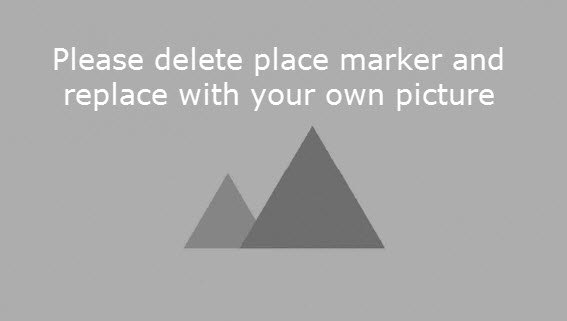
\includegraphics[scale=1.0]{images/placemarker.jpg}			% define cover picture
\end{textblock}

\begin{textblock}{154}(28,135)
	\begin{picture}(150,2)
		\put(0,0){\color{bfhgrey}\rule{150mm}{2mm}}
	\end{picture}
\end{textblock}
\color{black}

% Institution / titel / subtitel / authors / experts:
%---------------------------------------------------------------------------
\begin{flushleft}

\vspace*{115mm}

\fontsize{26pt}{28pt}\selectfont
\heading				\\							% Read heading from file leader/title.tex
\vspace{2mm}

\fontsize{16pt}{20pt}\selectfont\vspace{0.3em}
Informatik Seminar 			\\				% Insert subheading
\vspace{5mm}

\begin{textblock}{150}(28,225)
\fontsize{10pt}{17pt}\selectfont
\begin{tabbing}
xxxxxxxxxxxxxxx\=xxxxxxxxxxxxxxxxxxxxxxxxxxxxxxxxxxxxxxxxxxxxxxx \kill
Degree course:	\> Computer Science	\\		% insert name of degree course
Authors:		\> Anna Doukmak, Rajina Kandiah		\\					% insert names
Group:			\> 23\\
Tutor:	\> Simon Kramer		\\							% insert names
Date:			\> \versiondate					\\							% read from file leader/version.tex
\end{tabbing}

\end{textblock}
\end{flushleft}

\begin{textblock}{150}(28,280)
\noindent
\color{bfhgrey}\fontsize{9pt}{10pt}\selectfont
Berner Fachhochschule | Haute \'ecole sp\'ecialis\'ee bernoise | Bern University of Applied Sciences
\color{black}\selectfont
\end{textblock}


\end{titlepage}

%
% ===========================================================================
% EOF
%
		% activate for frontpage with picture
%% Control of versions :
% -----------------------------------------------

\begin{textblock}{180}(15,150)
\color{black}
\begin{huge}
Versions
\end{huge}
\vspace{10mm}

\fontsize{10pt}{18pt}\selectfont
\begin{tabbing}
xxxxxxxxxxx\=xxxxxxxxxxxxxxx\=xxxxxxxxxxxxxx\=xxxxxxxxxxxxxxxxxxxxxxxxxxxxxxxxxxxxxxxxxxxxxxx \kill
Version	\> Date	\> Status			\> Remarks		\\
0.1	\> 01.08.2013	\> Draft		\> Lorem ipsum dolor sit amet	\\	
0.2	\> 21.08.2013	\> Draft		\> Phasellus scelerisque	\\ 
0.3	\> 02.09.2013	\> Draft		\> Donec eget aliquam urna. Lorem ipsum dolor sit amet	\\ 
1.0	\> 26.01.2014	\> Final		\> Lorem ipsum dolor sit ametPhasellus scelerisque, leo sed iaculis ornare 	\\ 
1.1	\> 31.01.2014	\> Correction	\> Layout changed	\\
1.2	\> 07.02.2014	\> Addition		\> Chapter 1.1 extended	\\
\end{tabbing}

\end{textblock}

\cleardoubleemptypage
\setcounter{page}{1}
\cleardoublepage
\phantomsection
\addcontentsline{toc}{chapter}{Management Summary}
\chapter*{Abstract}
\label{chap:abstract}
The Transport Layer Security (\gls{tls}) is used for secured and encrypted communication over the networks. 2018 was the release date of the new \gls{tls} 1.3 which is defined in RFC8446. In this study we are going to figure out, what is new, what the changes to \gls{tls} 1.2 exactly are and what has remained the same. 

The questions of the particular improvement and the consequences, for example of the configurations or security will be identified. What was removed will also be noted and explained.

The first part of the study will give a brief overview about \gls{tls} and the different protocols. This part will give an overall explanation of how the process of the securing and encryption of the communication works. 

The main part will be the comparison of \gls{tls} 1.3 and \gls{tls} 1.2. This will be realised with the comparison of the changes. Namely the handhsake protocol, the session ressumption, the key derivation and supported ciphersuites which will be faced and analysed.

The conclusion will give a general overview based on the gathered information from the comparison.




\cleardoubleemptypage
%---------------------------------------------------------------------------

% Table of contents
%---------------------------------------------------------------------------
\tableofcontents
\cleardoublepage
%---------------------------------------------------------------------------

% Main part:
%---------------------------------------------------------------------------
\pagenumbering{arabic}

\chapter{Introduction}
\label{chap:introduction}

Transport Layer Security (\gls{tls}) Protocol is a cryptographic protocol that provides secure transport connection between applications over a computer network, e.g. web server and web browser. 
Using \gls{tls} prevents eavesdropping, tampering and message forgery. It provides privacy and data integrity between communicating applications. The protocol secures transmitted data using encryption. Secure communication with Authenticated Key Etablishment (\gls{ake}) and secure channel with Authenticated Encryption (\gls{ae}). 
Using Datagram \gls{tls} (\gls{dtls}) the stateless \gls{tls} is feasible. It offers server and, optionally, client authentication to confirm the identities of parties involved in the communication. 
 
Further, the integrity check value implemented in the protocol provides integrity for the transferred data. \gls{tls} is also known or referred to as Secure Socket Layer (\gls{ssl}), its predecessor. 
 
To use \gls{tls} all communicators must know that the other is supporting \gls{tls}.

\gls{tls} 1.2 was defined in \gls{rfc}5246 in August 2008. Its successor \gls{tls} 1.3 is defined in \gls{rfc}8446 in August 2018.
 \cite{RFC5246}\cite{ms:overview}

\section{Structure of the \gls{tls} Protocol}
\label{sec:stucture}

The \gls{tls} Protocol is layered between the Application layer and the TCP/IP layer according to the Internet Model (or between Session and Transport layers according to the OSI Model), where it can secure and then send application data to the transport layer \cite{ms:overview}. Thus it can support multiple application layer protocols, such as HTTP, FTP, SMTP, POP3. The protocols using \gls{tls} become respectively HTTPS, FTPS, SMTPS, POP3S and so on.

The \gls{tls} Protocol can be split into two layers. The lower layer of the \gls{tls} is the Record Protocol. The upper layer is the Handshake layer which consists of the following protocols: Handshake Protocol, ChangeCipherSpec Protocol and Alert Protocol. Figure \ref{fig:tls_structure} illustrates the structure of the \gls{tls} Protocol. 
\cite{tlsstrukt}

\begin{figure}[H]
	\centering
		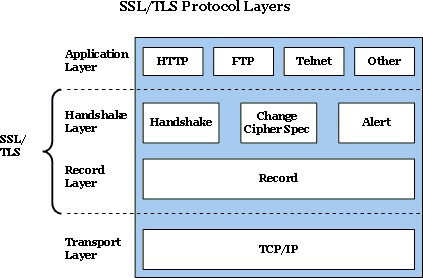
\includegraphics[scale=1]{images/tls_structure.jpg}
	\caption{\gls{tls} 1.2 Protocol Structure \cite{ms:overview}}
	\label{fig:tls_structure}
\end{figure}

\section{Handshake Protocol}
\label{sec:handshake_protocol}
 A handshake is an automated process of negotiation between communicators. The \gls{tls} Handshake Protocol is the most widely-used \gls{ake} Protocol to negotiate session information between the client and the server. 
 After the establishment of the TCP connection between a client and a server the handshake protocol will be triggered. 
 Thus, the purpose of this protocol is to negotiate and define these parameters:
 
 \begin{itemize}
\item to authenticate the server and optionally also the client
 \item to agree on the version of the \gls{tls}
 \item to have an agreement of the cipher suites
 \item to arrange with the extension
 \item to derive authenticated encryption key for the connection
 \item if required, to verify the certificates
 \item finally these all points also have to be assured between each communicators
\end{itemize}

To protect data, these parameters are then used by the record layer. As mentioned, usually it is only the server which is authenticated, but once a secure channel is established, the mutual authentications may also be carried out. This is permitted with the use of renegotiation, but requires a public key infrastructure (PKI). 
\cite{ms:overview}
\cite{ms:handshake}

\section{ChangeCipherSpec Protocol}
\label{sec:changeciphfer_protocol}
This protocol is responsible for informing about a change of one set of keys to another. It means that a transition in ciphering would be signaled through this protocol. This message is either sent by the server and client. 

This protocol triggers an instruction to the record layer.

The keying material is raw data which is used for encryption between the client and server. On the basis of the exchanged information from the handshake protocol, the keys will be then computed.
The ChangeCipherSpec Protocol consists of a byte with value 1.
The ChangeCipherSpec Protocol also includes a message to inform other parties in the \gls{ssl}/\gls{tls} session about the change.   \cite{ms:overview}

The ChangeCipherSpec protocol is removed from the 1.3 version of the \gls{tls} protocol.
\cite{WikipediaCipher}
\section{Alert Protocol}
\label{sec:alert_protocol}
The peer will be notified by the alert messages about the change in status or error condition (fatal/warning).These messages are also compressed and encrypted. If a fatal error occurs, the session will close immediately.
Fatal:
\begin{itemize}
	\item unexpected\_message
	 \item bad\_record\_MAC
	 \item handshake\_failure 
	 \item et al.
\end{itemize}
	
Warning:
\begin{itemize}
\item close\_notify
\item unsupported\_certificates
\item certificate\_expired
\item et al.

\end{itemize}

The full list of the alerts to notify the peer of normal or error condition is declared in \gls{rfc}2246 \cite{rfc2246}. All these alerts consists of 2 bytes. The first byte defines the kind (eg. fatal or warning) and the second specifies what happened \cite{W.Stalling} \cite{ms:overview}

\section{Record Protocol}
\label{sec:record_protocol}

The connection of two independent channels is established through the \gls{tls} Handshake, from the client to the server and in the other direction from the server to the client. The Record Protocol is responsible for the data protection on these channels using the authenticated encryption scheme.\\
The responsibilities of the Record Protocol are:
\begin{itemize}
	\item fragmentation
	\item compression
	\item application of MAC and encryption
	\item transmisson 
\end{itemize}
But the tasks/responsibilities depend also on the parameters of the keys, namely how the keys were set during the handshake protocol. \\
The processing of data is illustrated and described below:      

\begin{figure}[H]
	\centering
		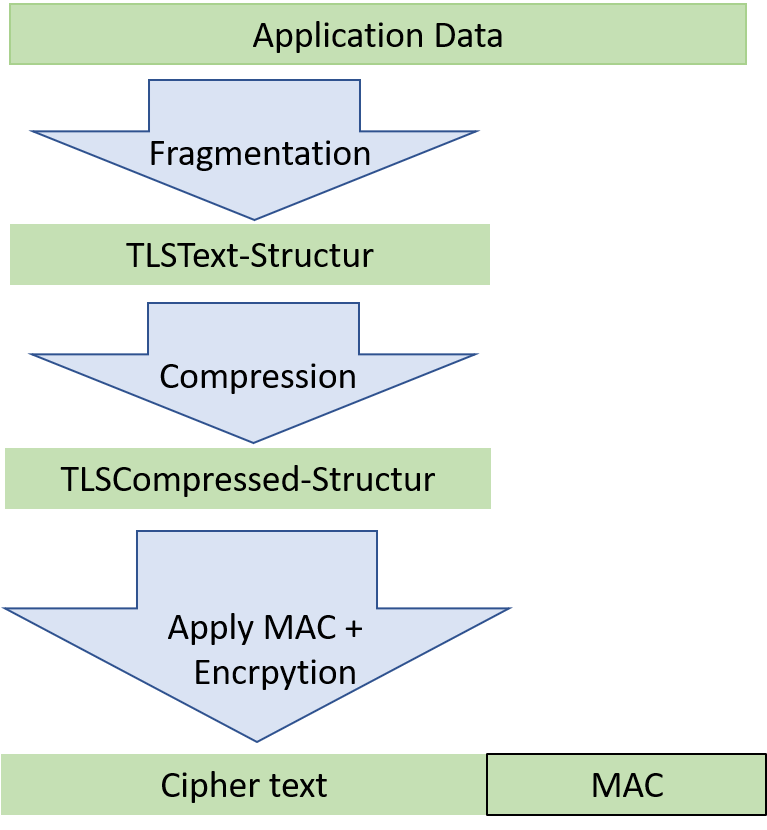
\includegraphics[scale=0.5]{images/tls_recordprotocol.png}
	\caption{\gls{tls} Record Protocol}
	\label{fig:tls_recordprotocol}
\end{figure}

First the Record Protocol layer receives the data from the application layer. Then it fragments the data to a size appropriate for the cryptographic algorithm. 
The next step is the compression, which is done if specified. The compression algorithm would then be defined in the current session state and would translate the date to a TLSCompressed structure.
 
Subsequently the message authentication code over the compressed data would be computed.
To ensure that the data were not altered during the transmission, the MAC value is added. So the receiver can check if the incoming MAC value and the computed one 
match. Thus, the integrity and confidentiality are ensured.

As a hint, the first handshake is neither secured by a MAC nor encrypted. Because this is the initial value for the keys, it is how they are first set. After the first handshake these parameters are set and therefore secured and encrypted.
\cite{ms:Record} \cite{Hassenstein}
\chapter{Comparative Study}
\label{chap:comparative_study}

The version 1.2 of the TLS protocol was defined in RFC5246 in August 2008 und has been in use many years. With the release of TLS 1.3 in August 2018 some security and speed improvements of the protocol have been implemented. The TLS 1.3 is defined in RFC8446. In the following chapters the changes and differences of both TLS releases are examinated and discussed.

\section{Comparison of the handshake protocol}
\label{sec:comparison_handshake}

As described in the chapter ... (todo: add reference) the Handshake begins after the establishment of the TCP connection between client and server. The goals of the handshake protocol are to authenticate the server and, optionally, the client; negotiate protocol version, ciphersuites and extensions; derive authencticated encryption keys for the secure connection; ensure agreement on all negotiated parameters. \cite{Hassenstein}

\subsection{TLS 1.2 handshake}
\label{subsec:handshake1_2}

The figure \ref{fig:handshake1_2} shows the process of the full handshake in the TLS protocol 1.2 for simplicity only with authentication of the server. There will be more steps of the handshake in case of the mutual authentication when the client must be also authenticated by the server.

\begin{figure}[H]
	\centering
		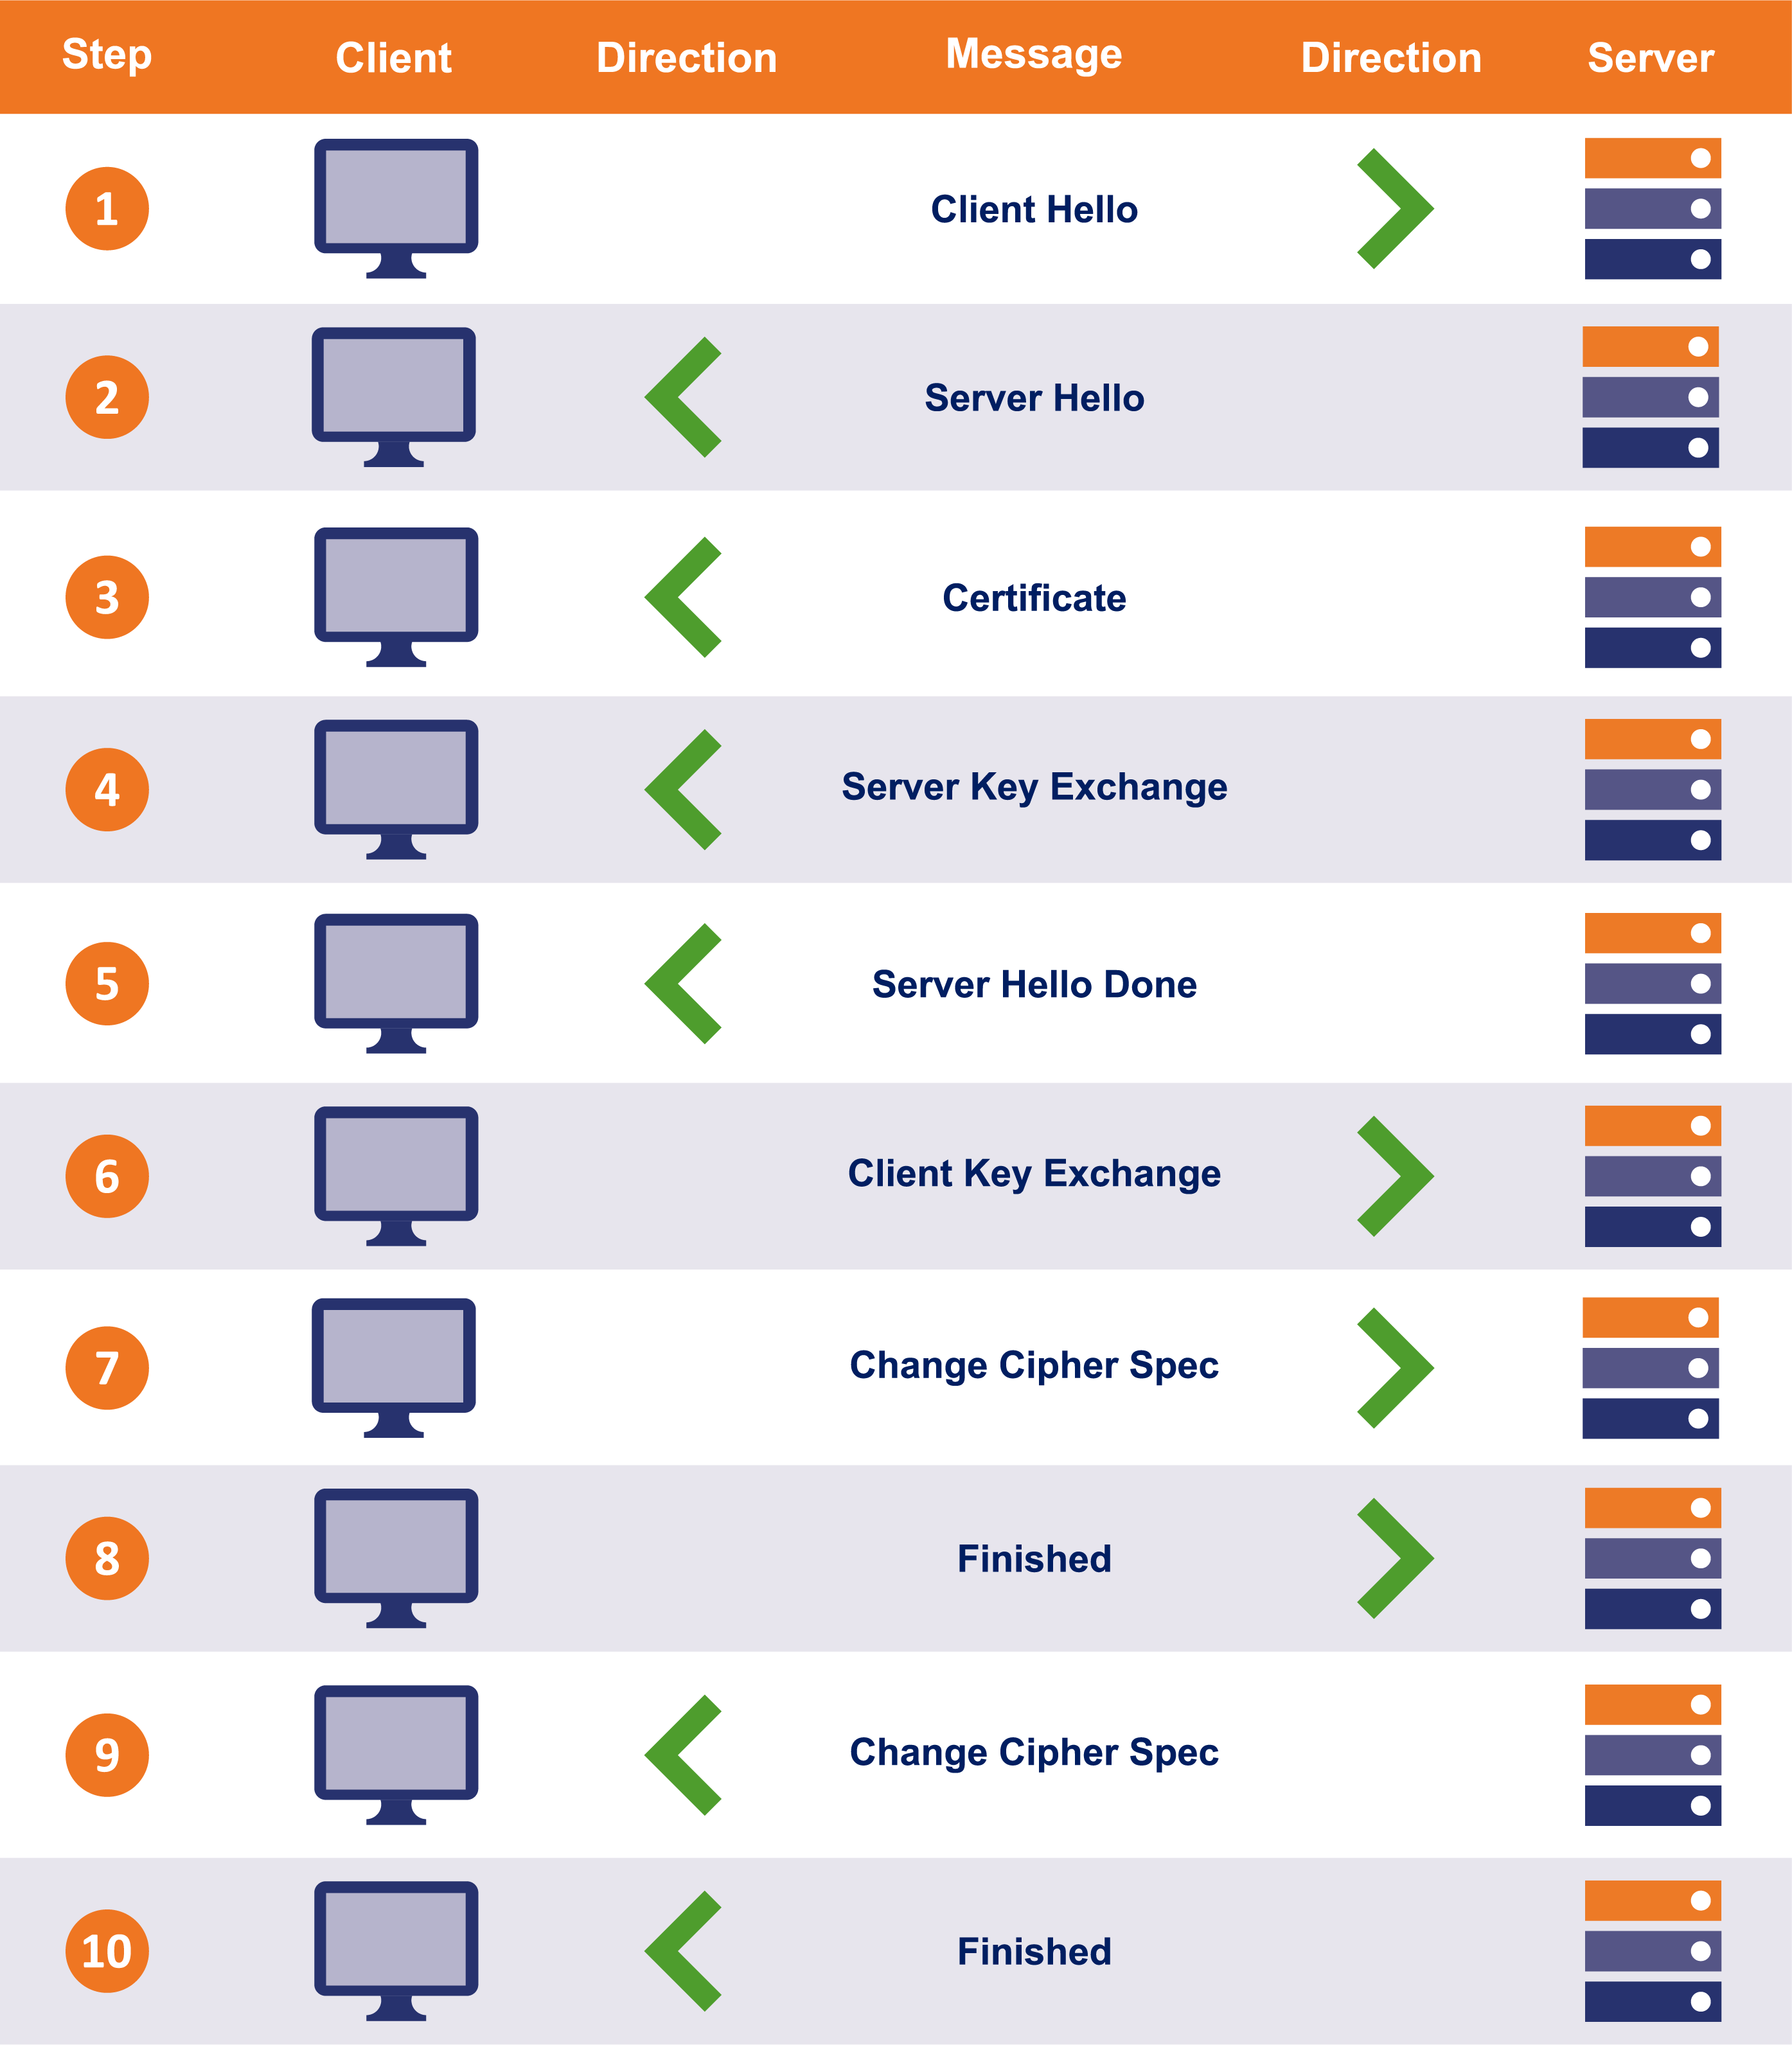
\includegraphics[scale=0.35]{images/handshake1_2.png}
	\caption{TLS 1.2 full handshake \cite{sslstore:handshake}}
	\label{fig:handshake1_2}
\end{figure}

\textbf{Step 1.} The 1th round of the handshake begins with the "client hello" message sent from the client to the server. This message includes the following cryptographic information:

\begin{itemize}
	\item CipherSuites - encryption algorithms supported by the client
	\item desired maximum of the protocol version
	\item random value generated on the client side
	\item session id
\end{itemize}

\textbf{Step 2.} Then the server responds with "server hello" message. The message consists of the following information:

\begin{itemize}
	\item CipherSuites chosen by the server from the "client hello" message
	\item protocol version supported by the server
	\item random value generated on the server side
	\item session id
\end{itemize}

\textbf{Step 3.} The server sends its X.509 certificate and its public key.

\textbf{Step 4.} This step is needed if the Diffie-Hellmann key exchange algorithm was negotiated between the client and the server at the steps 1 and 2. In this case the server transmits additional key materials in the "server key exchange" message.

\textbf{Step 5.} With the "server hello done" message the server notify the client that it finished his steps and wait on the answer of the client.

\textbf{Step 6.} The client verifies the certificate sent by the server. Then it transmit to the server its key material in the key exchange message. 
At this point the client and the server can compute pre-master secret from key exchange messages. Using the pre-master secret with the nonces sent in the steps 1 and 2 they can generate the master key. Afterwards the client and the server derive a set of session keys from the master key that will be used to symmetrically encrypt the data.

\textbf{Step 7.} Wenn the client derived the session key it notify the server about the change of the keys for the secure communication.

\textbf{Step 8.} With the message "Finished" the client signals to the server that it completed its tasks and is ready for the communication. This message includes MAC of the messages from the previous steps using the calculated master key, so that the server can verify integrity of the handshake's messages.

\textbf{Step 9-10.} The server makes the same steps as the client in the steps 7-8 to switch the keys for the symmetric encryption and notifies the client with the message "finished". This message includes the MAC of the whole handshake log except "change cipher spec" messages from the steps 7 and 9. \cite{sslstore:handshake}\cite{Hassenstein}

The almost whole communication in the handshake protocol flows in the clear text. Only beginning from the step 8, when the client finished his preparation for the secure communication, the next messages of the handshake will be encrypted.

\subsection{TLS 1.3 handshake}
\label{subsec:handshake1_3}

\begin{figure}[H]
	\centering
		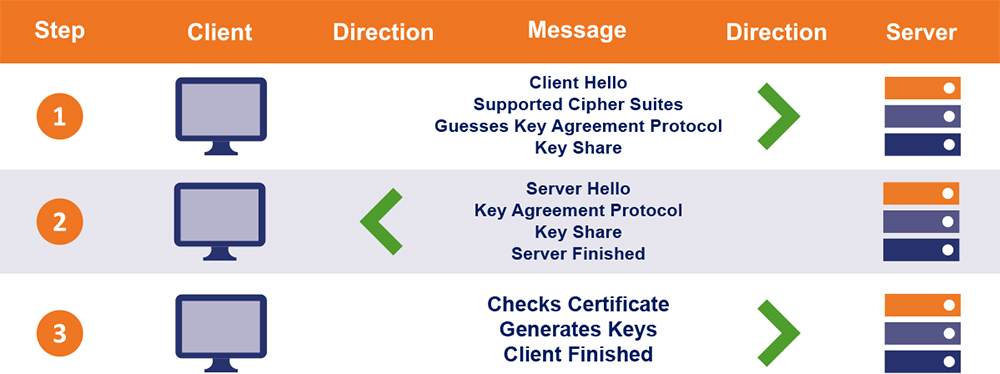
\includegraphics[scale=0.35]{images/handshake1_3.jpg}
	\caption{TLS 1.3 full handshake \cite{sslstore:handshake}}
	\label{fig:handshake1_3}
\end{figure}

\textbf{Step 1.} The TLS 1.3 handshake begins with the "client hello" message as in the TLS 1.2 handshake. In addition the client sends in the same message the following information:

\begin{itemize}
	\item the list of the supported CypherSuites
	\item key share entries consisting of a named (EC)DH group and an ephemeral public key
\end{itemize}

\textbf{Step 2.} The server respondes with the "server hello" message. In addition it sends the following information:

\begin{itemize}
	\item chosen CypherSuite
	\item key share entries consisting of the chosen (EC)DH group and its public key
	\item the certificate of the server
	\item "certificate verify" message containing a hash of all previous handshake messages signed with the private key of the server. The client afterwards verifies the signature with the public key from the server's certificate. 
	\item "server finished" message
\end{itemize}

In case if the server does not support any of the proposed groups the server will request retrying the handshake or abort the connection with a fatal handshake\_failure alert.

\textbf{Step 3.} The client checks the certificate of the server. Generates keys from the key share of the server from the previous step. Afterwards the client sends the "client finished" message. \cite{Hassenstein}\cite{sslstore:handshake}

After the "server hello" message all handshake messages will be encrypted.

\subsection{Discussion of TLS 1.2 and 1.3 full handshakes (todo: change title)}
\label{subsec:comparison_handshake}

The TLS 1.2 handshake takes two round trips between the client and the server to complete the handshake. On average, this process requires 0.25 to 0.5 seconds.

The "server key exchange" and "client key exchange" messages have been removed from the TLS 1.3 handshake. The key exchange parameters and public keys will be sent in the key share extensions, that are added to the "client hello" and "server hello" messages. This keeps the 1.3 release compatible with the 1.2 version because the order of messages remains.

Furthermore the ChangeCipherSpec protocol has been removed in the 1.3 version. 

As a consequence of this the TLS 1.3 handshake involves only one round trip. This changes results in reduced latency almost in half. As mentioned in the blog of The SSL Store a delay of half a second results in 20\% traffic decline \cite{sslstore:handshake}. That is why the performance improvement of the TLS protocol is a crucial change in the protocol.

Moreover the privace of the handshake protocol has been improved. In the 1.2 release of the TLS protocol almost all handshake messages are sent in the clear text except the last steps after the client sends "finished" message. On the contrary in the 1.3 version all information will be encrypted as early as possible, namely after "server hello" message. 

\section{Comparison of the session resumption}
\label{sec:comparison_resumption}

The full handshake can take time, increase server load and cause connection latency. To improve performance the session resumption can be used. With the "client hello" and "server hello" messages the session id can be saved and used to resume previously established TLS session. Under this session id the client and the server store the master key and other details of the connection. In the next session they can transmit the session id and thus reuse past connection parameters. The following session data can be cached: master secret, protocol version, ciphersuits, compression method, certificate. Because the session resumption is efficient it is supported per dafault in all major web browsers and web servers. But if it is not correctly implemented that can lead to vulnerabilities.

\subsection{Session resumption in TLS 1.2}
\label{subsec:resumption1_2}

The client and the server can set up a new connection by reusing the master key from the recent session cached on both ends in the one rount-trip handshake. This kind of handshake is called abbreviated TLS handshake. The figure \ref{fig:resumption1_2} illustrates the process of the abbreviated handshake for the session resumption in the TLS 1.2.

\begin{figure}[H]
	\centering
		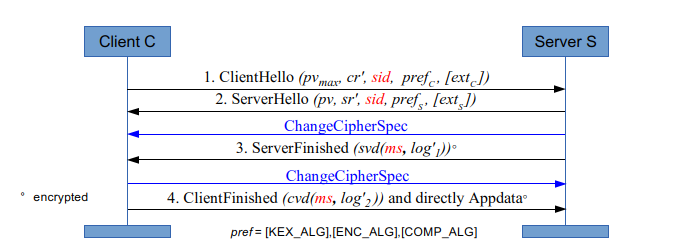
\includegraphics[scale=0.85]{images/resumption1_2.png}
	\caption{Abbreviated Handshake for Session Resumption in TLS 1.2 \cite{Hassenstein}}
	\label{fig:resumption1_2}
\end{figure}

In the "client hello" message the client sends to the server the session id from which the connection parameter can be used. As well a new random value (nonce) should be transmitted by the client. If the session with his session id has been cached the server respons in the "server hello" message with a new nonce and the same CipherSuites as in the previous handshake. Without waiting for the client's answer the server immediatly notifies the client about the changes of the key with the ChangeCipherSpec message and finishes its part of the handshake with MAC of the abbreviated handshake log in the encrypted "server finished" message. The client answers with its notification about the change of the key and completes the handshakes process with the "client finished" message containing a MAC of the whole abbreviated handshake log with the exception of ChangeCipherSpec messages. The both parties use the master key from the previous handshake and the new nonces to derive a set of session keys for the symmetric encryption of their communication.

The session resumption is also possible with the session ticket. In this case the client transmits the session ticket in the "client hello" message instead of the session id. The session ticket is a blob file created by the server and stored on the client side. This file contains all necessary detail of a connection and is encrypted with the key only known to the server. After the decryption of the ticket by the server the master key will be resumed for the derivation of session keys.

Figure \ref{fig:without-with-resume-1_2} demonstrates the efficiency of the session resumption. The abbreviated handshake is almost in half faster than the full handshake.

\begin{figure}[H]
	\centering
		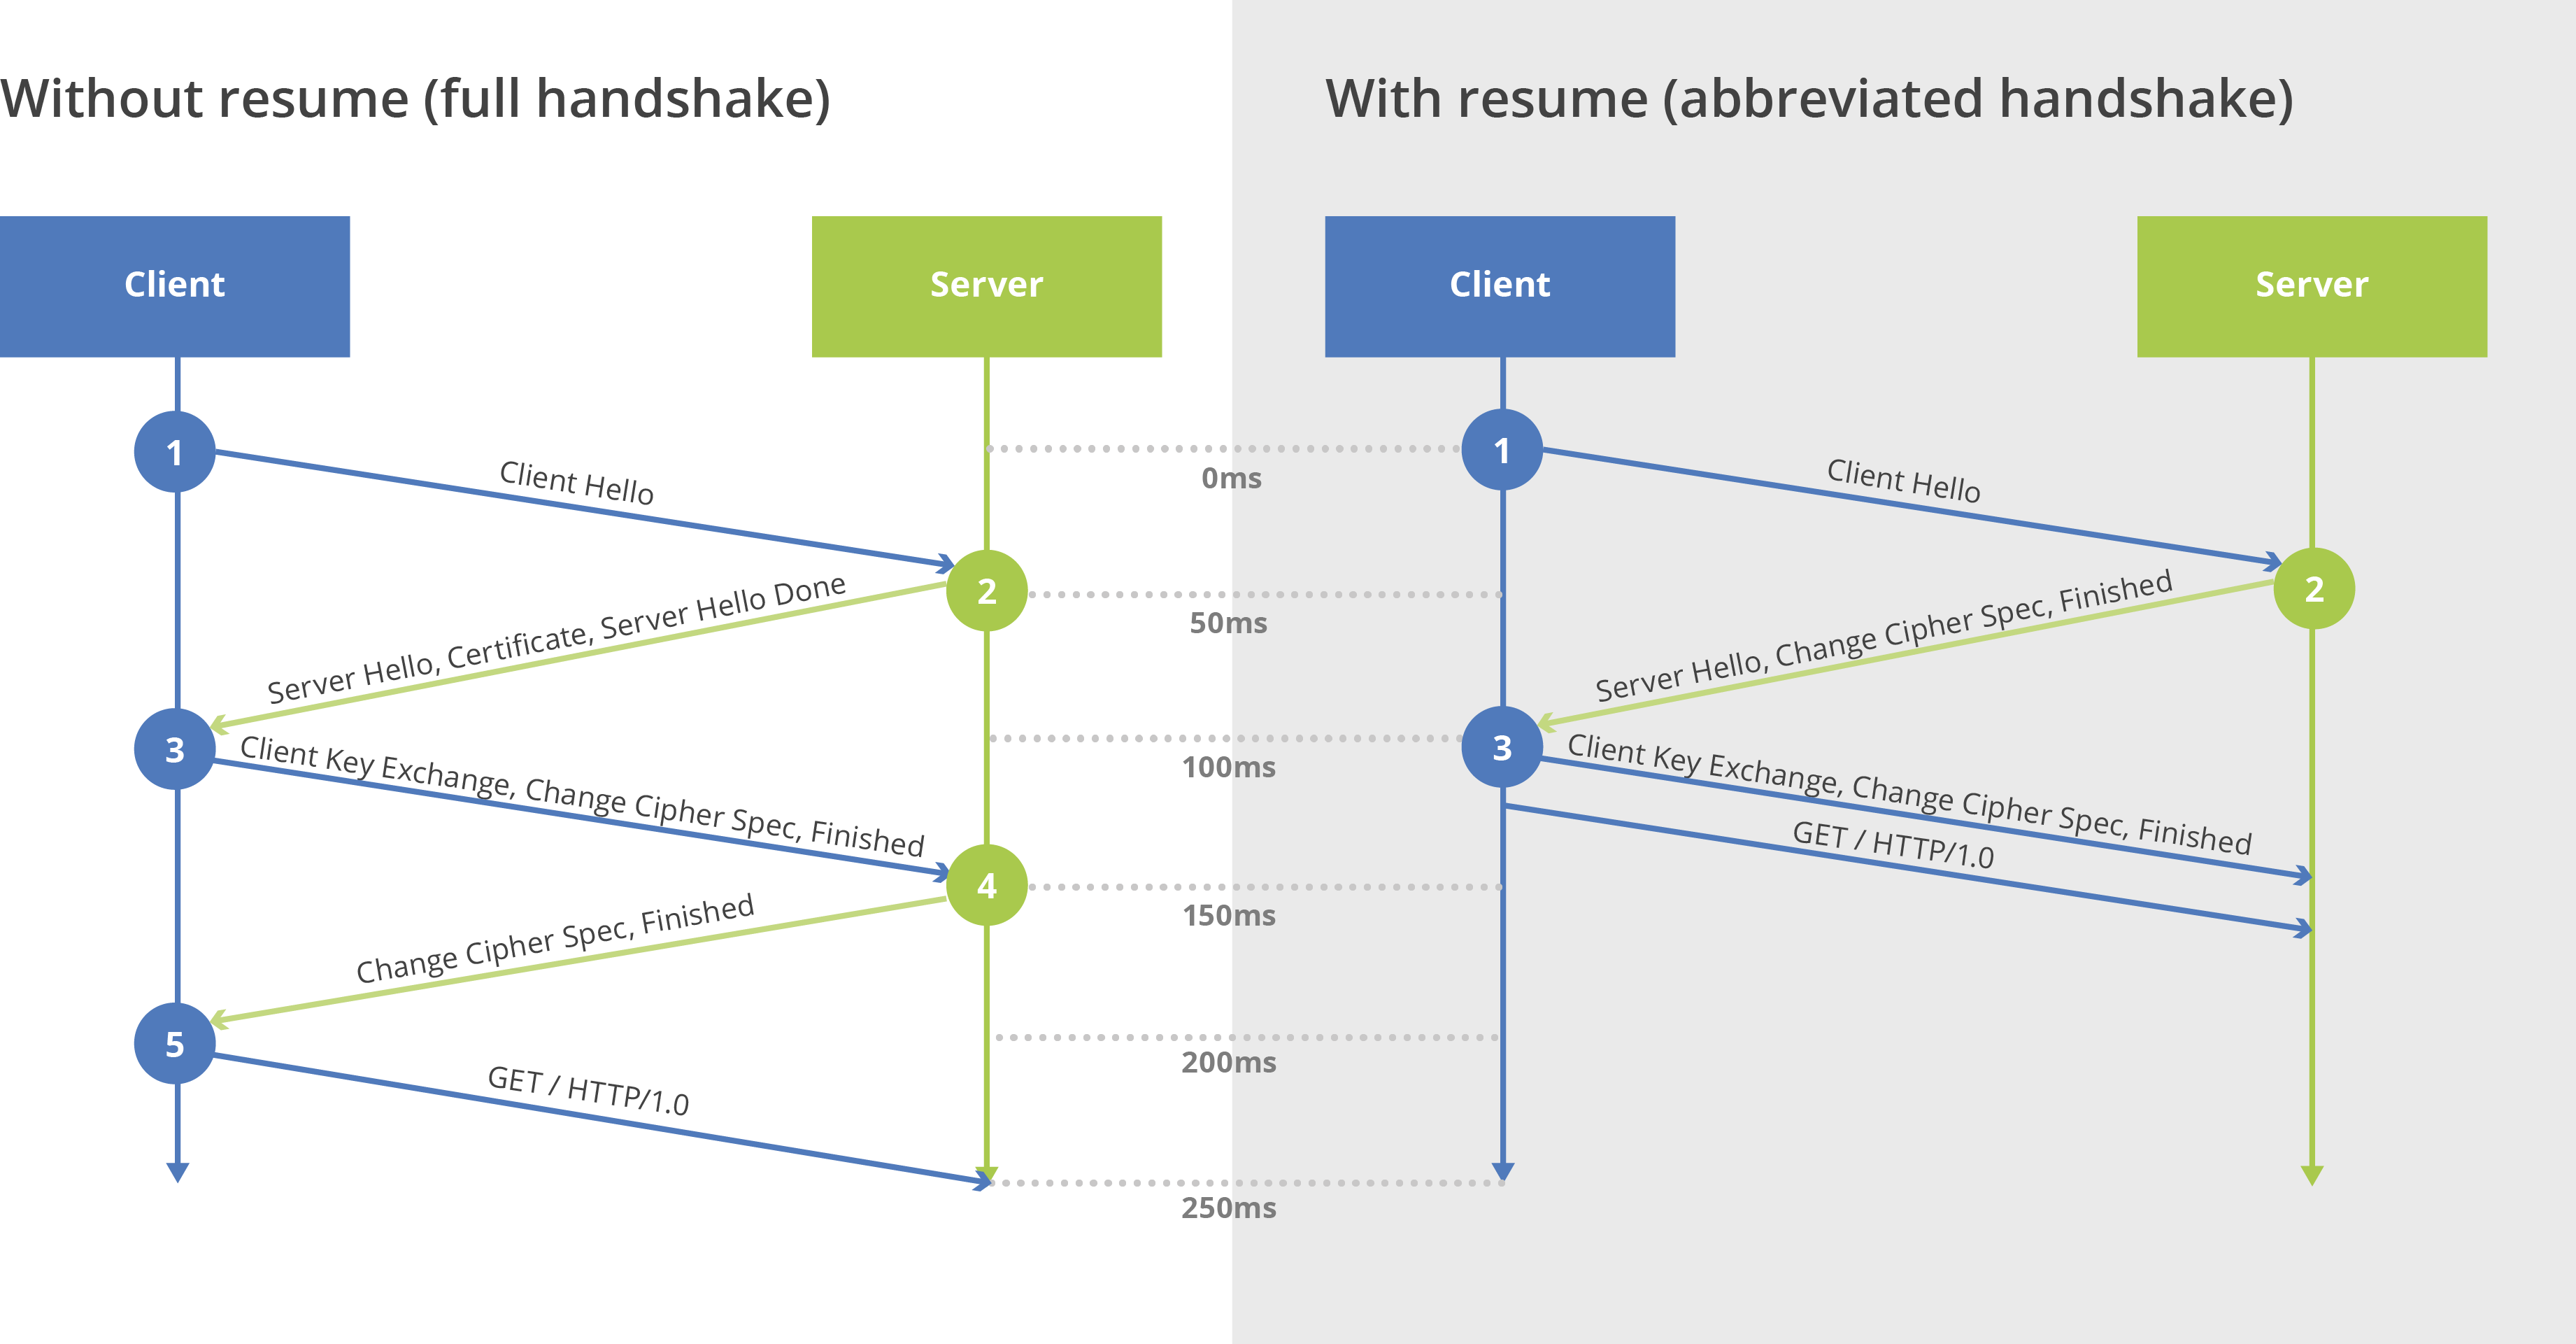
\includegraphics[scale=0.4]{images/without-with-resume-1_2.png}
	\caption{Full TLS handshake vs. abbreviated TLS handshake \cite{cloudflare:resume}}
	\label{fig:without-with-resume-1_2}
\end{figure}

\subsection{Session resumption in TLS 1.3}
\label{subsec:resumption1_3}

There are differences how the sesssion resumption works in the release 1.3 of TLS. Figure \ref{fig:resumption1_3} illustrates the process of the handshake for the session resumption in TLS 1.3.

\begin{figure}[H]
	\centering
		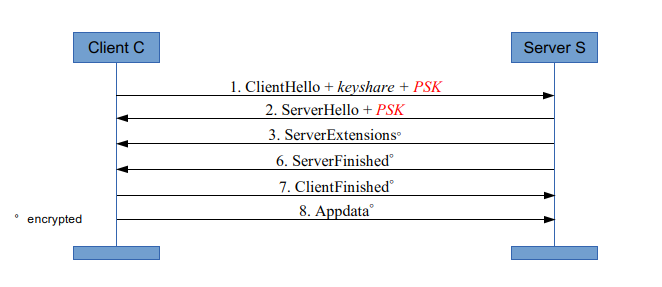
\includegraphics[scale=0.8]{images/resumption1_3.png}
	\caption{Handshake for Session Resumption in TLS 1.3 \cite{Hassenstein}}
	\label{fig:resumption1_3}
\end{figure}

A new method to resume the session is implemented in TLS 1.3. It is called pre-shared key (PSK) mode and replaces the usage of the session identifier or session ticket. An PSK identity is sent to the client by the server after the full handshake is completed. The PSK identity is a blob file containing database lookup keys or self-encrypted and self-authencitcated values. It corresponds to a key derived from the handshake.

A PSK, that has been created during the handshake of the prevoius connection, can be presented by the client on the next visit. If it is needed to resume the session the client transmits PSK identities to the server. Then the server responds with the chosen PSK identity in the "server hello" message. The security context of this identity will be used in the new connection and the unique key derived from the previous connection can be used in the new one. \cite{ldapwiki:resumption}

\subsection{Discussion of the session resumption in TLS 1.2 and 1.3}
\label{subsec:discussion_resumption}

\section{Comparison of cipher suits}
\label{sec:comparison_ciphersuits}

\section{Comparison of key derivation funcitons}
\label{sec:comparison_kdf}

\section{Connection renegotiation}
\label{sec:comparison_renegotiation}

\section{Overview}
\label{sec:overview}

\begin{table}[H]
	\centering
		\begin{tabular}{lll} \toprule
			\textbf{Characteristic} & \textbf{TLS 1.2} & \textbf{TLS 1.3} \\ \midrule
			Round trip time of the full handshake & 2-RTT & 1-RTT \\ \midrule
			Encryption of handshake messages& at the end, & at the beginning, \\ 
			& from "client finished" message & after "server hello" message \\ \midrule
			Performance of the full handshake & 0.25-0.5 s & 0.2-0.3 s\\ \midrule
			Round trip time of the handshake & 1-RTT & 0-RTT \\ 
			for session resumption \\ \midrule
			Session resumption method & session id or session ticket & pre-shared key identity \\ \midrule
		\end{tabular}
	\caption{Comparison of TLS 1.2 and TLS 1.3}
	\label{tab:comparison}
\end{table}


\chapter{Conclusion}
\label{chap:conclusion}





%---------------------------------------------------------------------------

% Selbst�ndigkeitserkl�rung
%---------------------------------------------------------------------------
\cleardoublepage
\phantomsection
\addcontentsline{toc}{chapter}{Declaration of authorship}
\chapter*{Declaration of primary authorship}
\label{chap:declaration_authorship}

\vspace*{10mm} 

We hereby confirm that we have written this thesis independently and without using other sources and resources than those specified in the bibliography. All text passages which were not written by me are marked as quotations and provided with the exact indication of its origin. 

\vspace{15mm}

\begin{tabbing}
xxxxxxxxxxxxxxxxxxxxxxxxxxxxxx\=xxxxxxxxxxxxxxxxxxxxxxxxxxxxxx\=xxxxxxxxxxxxxxxxxxxxxxxxxxxxxx\kill
Place, Date:		\> Biel, \versiondate \\ \\ 
Last Names, First Names:	\> Anna Doukmak 	\> Rajina Kandiah \\ \\ \\ \\ 
Signatures:	\> ......................................\> ...................................... \\
\end{tabbing}

%---------------------------------------------------------------------------

% Glossary
%---------------------------------------------------------------------------
\cleardoublepage
\phantomsection
\addcontentsline{toc}{chapter}{Glossary}
%\renewcommand{\glossaryname}{Glossary}
\printglossary
%---------------------------------------------------------------------------

% Bibliography
%---------------------------------------------------------------------------
\cleardoublepage
\phantomsection
\addcontentsline{toc}{chapter}{Bibliography}
\bibliographystyle{IEEEtranS}
\bibliography{database/bibliography}{}
%---------------------------------------------------------------------------

% Listings
%---------------------------------------------------------------------------
\cleardoublepage
\phantomsection
\addcontentsline{toc}{chapter}{List of figures}
\listoffigures
\cleardoublepage
\phantomsection
\addcontentsline{toc}{chapter}{List fo tables}
\listoftables
%---------------------------------------------------------------------------

% Index
%---------------------------------------------------------------------------
\cleardoublepage
\phantomsection
\addcontentsline{toc}{chapter}{Index}
\printindex
%---------------------------------------------------------------------------

% Attachment:
%---------------------------------------------------------------------------
\appendix
\settocdepth{section}
\chapter*{APPENDICES}
\addcontentsline{toc}{chapter}{APPENDICES}
\chapter{Technical Documentation}
\label{chap:appendix_tech_docu}

\chapter{Source Code}
\label{chap:appendix_source_code}

\chapter{Database Schema}
\label{chap:appendix_db_schema}

%---------------------------------------------------------------------------

%---------------------------------------------------------------------------
\end{document}

